\documentclass[10pt,a4paper]{article}
\usepackage[utf8]{inputenc}
\usepackage[italian]{babel}
\usepackage{amsmath}
\usepackage{amsfonts}
\usepackage{amssymb}
\usepackage{graphicx}
\usepackage[left=2cm,right=2cm,top=2cm,bottom=2cm]{geometry}
\newcommand{\rem}[1]{[\emph{#1}]}
\newcommand{\exn}{\phantom{xxx}}

\author{Gruppo 1G.BT \\ Lorenzo Cavuoti, Francesco Sacco}
\title{Es01B: Misure di tensione, corrente, tempi, frequenza.}
\begin{document}
\date{4 Ottobre 2018}
\maketitle

\setcounter{section}{1}
\section{Misure di tensione e corrente}

\paragraph{2.b Partitore con resistenze da circa 1~k}
Valori misurati $R_1$ e $R_2$ e valore atteso di $A_\mathrm{exp}$:
\[
R_1 = (1182 \pm 9) \,\Omega, \quad
R_2 = (971 \pm 7) \,\Omega, \quad
A_\mathrm{exp} = ( 0.452 \pm 0.004 ) 
\]


\begin{table}[h]
\centering
\begin{tabular}{|c|c|c|c|c|c|}
\hline 
VIN& $\sigma$ VIN  &VOUT	 & $\sigma$ VOUT& VOUT/VIN & $\sigma$ VOUT/VIN \\
\hline 
1,928 & 0,009 & 0,868 & 0,004 & 0.450 &\exn 0.005 \\
5,94 & 0,03 & 2,68 & 0,02 & 0.451 &\exn 0.005 \\
4,24 & 0,02 & 1,91 & 0,01 & 0.450 &\exn 0.005 \\
2,65 & 0,02 & 1,194 & 0,006 & 0.451 &\exn 0.005 \\
6,19 & 0,17 & 2,80 & 0,02 & 0.452 &\exn 0.005 \\
7,28 & 0,03 & 3,29 & 0,02 & 0.452 &\exn 0.005 \\
8,41 & 0,04 & 3,80 & 0,02 & 0.452 &\exn 0.005 \\
9,79 & 0,04 & 4,42 & 0,02 & 0.451 &\exn 0.005 \\
0,868 & 0,004 & 0,392 & 0,002 & 0.452 &\exn 0.005 \\
\hline 
\end{tabular} 
\caption{(2.b) Partitore di tensione con resistenze da circa 1k. Tutte le tensioni in V.\label{t:par1}}
\end{table}

\begin{figure}[h]
\centering
%\includegraphics[scale=0.4]{part1.pdf}
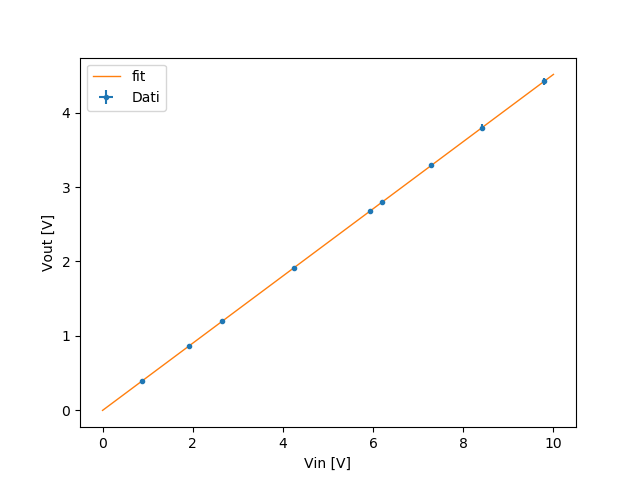
\includegraphics[scale=0.6]{plot_2b.png}
 

\caption{(2.b) Grafico $V_{out}$ vs. $V_{in}$ con resistenze di circa 1k \label{f:par1}}
\end{figure}

Risolvendo il circuito considerando un voltmetro ideale si trova $V_{out}/V_{in} = R_2/(R_1+R_2)$ quindi facendo il grafico di $V_{out}$ vs $V_{in}$ ci aspettiamo una retta passante per l'origine con coefficiente angolare $R_2/(R_1+R_2) = 0.451 \pm 0.006$. Eseguendo il fit con la funzione curve-fit di scipy e lasciando absolute-sigma=False, in quando gli errori non sono statistici, otteniamo un coefficiente angolare $a=0.4514\pm0.0004$ e un intercetta $b=(0.4\pm0.8)\times10^{-3}$, entrambi compatibili con le aspettative. 


\paragraph{2.c Partitore con resistenze da circa 4M}
Valori misurati $R_1$ e $R_2$ e valore atteso di $A_\mathrm{exp}$:
\[
R_1 = ( 3,80 \pm 0,04 ) \,\mathrm{M}\Omega, \quad
R_2 = ( 4,81 \pm 0,05 ) \,\mathrm{M}\Omega, \quad
A_\mathrm{exp} = ( 0.559 \pm 0.005 ) 
\]


\begin{table}[h]
\centering
\begin{tabular}{|c|c|c|c|c|c|}
\hline 
VIN& $\sigma$ VIN  &VOUT	 & $\sigma$ VOUT& VOUT/VIN & $\sigma$ VOUT/VIN \\
\hline 
0,754 & 0,003 & 0,347 & 0,002 & 0.460 & 0.005 \\
1,825 & 0,009 & 0,839 & 0,004 & 0.460 & 0.005 \\
2,89 & 0,02 & 1,332 & 0,007 & 0.461 & 0.005\\
4,150 & 0,02 & 1,910 & 0,010 & 0.460 & 0.005\\
5,26 & 0,03 & 2,42 & 0,01 & 0.460 & 0.005\\
7,02 & 0,04 & 3,24 & 0,02 & 0.461 & 0.005\\
8,13 & 0,04 & 3,74 & 0,02 & 0.460 & 0.005\\
9,23 & 0,05 & 4,25 & 0,02 & 0.460 & 0.005\\
6,17 & 0,03 & 2,48 & 0,02 & 0.460 & 0.005\\
\hline 
\end{tabular} 
\caption{(2.c) Partitore di tensione con resistenze da circa 4M. Tutte le tensioni in V.\label{t:par2}}
\end{table}


\begin{figure}[h]
\centering
%\includegraphics[scale=0.4]{part1.pdf}
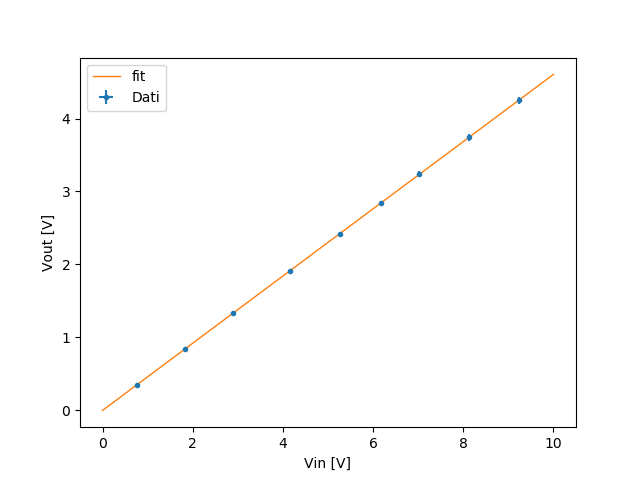
\includegraphics[scale=0.6]{plot_2c.png}

\caption{(2.c) Grafico $V_{out}$ vs. $V_{in}$ con resistenze da circa 4M \label{f:par2}}
\end{figure}

Anche in questo caso, considerando un voltmetro ideale, ci aspettiamo $V_{out}/V_{in} = R_2/(R_1+R_2)$, facendo il grafico di $V_{out}$ vs $V_{in}$ ci aspettiamo una retta passante per l'origine con coefficiente angolare $R_2/(R_1+R_2) = 0.557 \pm 0.007$. Eseguendo il fit con la funzione curve-fit di scipy e lasciando absolute-sigma=False in quando gli errori non sono statistici si trova un coefficiente angolare $a=0.4605\pm0.0003$ e un intercetta $b=(0.3\pm0.5)\times10^{-3}$. Nonostante l'intercetta sia compatibile con le aspettative il coefficiente angolare è molte barre di errore all'infuori del valore misurato, ciò potrebbe essere dovuto al fatto che il nostro voltmetro non sia ideale e di conseguenza ha resistenza interna molto grande ma finita.


\paragraph{2.d Resistenza di ingresso del tester}
Usando il modello mostrato nella scheda si ottiene
\[ \frac{R_1}{R_T} =  \frac{V_{IN}}{V_{OUT}} - (1 +  \frac{R_1}{R_2} )
\]

Con i dati del punto 2.b si ottiene
\[ R_1/R_T = 0.00  \pm  0.01   \rightarrow  R_T > 100 k\Omega
\]


Con i dati del punto 2.c si ottiene
\[ R_1/R_T = 0.38  \pm  0.01   \rightarrow  R_T = ( 9.9\pm  0.3)  M\Omega
\]

Usando resistenze da circa $1 k\Omega$ il rapporto $R_1/R_T$ risulta compatibile con 0, tuttavia, sappiamo che $R_1/R_T$ è un numero strettamente maggiore di 0 e minore di 0.01, di conseguenza si può porre un limite inferiore alla resistenza del tester: $R_T>100 k\Omega$. Aumentando i valori delle resistenze nell'ordine dei $4M\Omega$ si ottiene $R_1/R_T = 0.38  \pm  0.01$, non più compatibile con 0, questo ci permette di stimare $R_T$ con un errore relativo del $3\%$


\section{Uso dell'oscilloscopio}

\paragraph{3.b Misure di tensione} 
Vengono ripetute le misure del punto 2.c  ma con pochi punti e senza grafico
\begin{table}[h]
\centering
\begin{tabular}{|c|c|c|c|c|c|}
\hline 
VIN& $\sigma$ VIN  &VOUT	 & $\sigma$ VOUT& VOUT/VIN & $\sigma$ VOUT/VIN \\
\hline 
1,68 & 0,07 & 0,30 & 0,01 & 0.17 & 0.01\\
3,72 & 0,15 & 0,68 & 0,03 & 0.18 & 0.01 \\
7,44 & 0,3 & 1,28 & 0,05 & 0.17 & 0.01 \\
9,8 & 0,4 & 1,76 & 0,07 & 0.18 & 0.01 \\
\hline 
\end{tabular} 
\caption{(3.b) Partitore di tensione con resistenze da circa 4M, misura con oscilloscopio. Tutte le tensioni in V.}
\end{table}


\paragraph{3.d Impedenza di ingresso dell'oscilloscopio} Si ripete l'analisi del punto 2.d

\[ R_1/R_{IN} = 3.86 \pm  0.01   \rightarrow  R_{IN} = (0.98 \pm  0.01)  M\Omega
\]


\section{Misure di frequenza e tempo}

\paragraph{4.b Misure di frequenza}
Misure con onda sinusoidale
\begin{table}[h]
\centering
\begin{tabular}{|c|c|c|c|c|c|}
\hline 
Periodo T (s)& $\sigma$ T (s)  &Frequenza f (Hz) & $\sigma$ f (Hz) & Misura oscilloscopio (Hz) & Differenza (Hz)\\
\hline 
1,01 \times 10^{-3} & 0,01 \times 10^{-3} & 990 & 10 & 997 &7 \\
1,02 \times 10^{-4} & 0,01 \times 10^{-4}& 9,8 \times 10^3 & 0,1 \times 10^3 & 9,9\times10^3 &10^2 \\
1,00 \times 10^{-5} &0,01 \times 10^{-5}& 1,0 \times 10^5 & 0,01 \times 10^5  & 9,99\times10^4 &10^2\\
1,01 \times 10^{-6} &0,01 \times 10^{-6}& 9,90 \times 10^5 & 0,1 \times 10^5 & 1,00\times 10^6 &10^5 \\
\hline 
\end{tabular} 
\caption{(4.b) Misura di frequenza di onde sinusoidali  e confronto con misurazione interna dell'oscilloscopio }
\end{table}



\section{Trigger dell'oscilloscopio}
\paragraph{5.b Segnale pulse}
Misure con segnale pulse del generatore di onde
\begin{figure}[h]
\centering
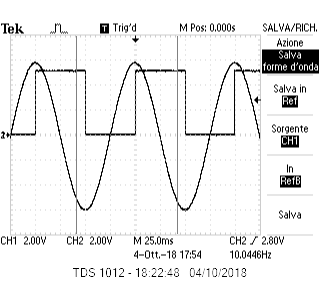
\includegraphics[scale=0.9]{screen_osc.png}
\caption{(5.b) Relazione temporale tra il segnale pulse e l'onda principale}
\end{figure}


\section{Conclusioni e commenti finali}
Nel caso di resistenze da 1k il valore del coefficiente angolare misurato è in accordo con quello atteso, mentre per resistenze più elevate questo non è valido. Tuttavia questa discrepanza può essere giustificata considerando la resistenza interna del voltmetro. Inoltre, sfruttando la differenza tra valore misurato e atteso siamo riusciti a stimare la resistenza interna del multimetro digitale per misure di ddp, che risulta $R_T = ( 9.9\pm  0.3)  M\Omega$. Inoltre, con lo stesso metodo, abbiamo misurato anche la resistenza interna dell'oscilloscopio che risulta $R_{IN} = (0.98 \pm  0.01)  M\Omega$. \\\\
Nelle misure della frequenza con  l'oscilloscopio, confrontando il valore della frequenza per segnali sinusoidali letti dall'oscilloscopio e la nostra stima (calcolata misurando il periodo dell'onda e facendo l'inverso) notiamo che i valori sono compatibili, entro una barra di errore, per tutte le frequenze in esame. Tuttavia, il fatto che la misura di frequenza che esegue l'oscilloscopio non ha errore e non sappiamo bene ne come calcolarlo ne come funziona l'algoritmo che calcola la frequenza, non possiamo usare questo metodo per fare misure. Inoltre, pur funzionando bene per segnali sinusoidali, non possiamo essere sicuri che calcoli adeguatamente la frequenza per altri tipi di segnali.

\section*{Dichiarazione}
I firmatari di questa relazione dichiarano che il contenuto della relazione \`e originale, con misure effettuate dai membri del gruppo, e che tutti i firmatari hanno contribuito alla elaborazione della relazione stessa.

\end{document}